\begin{figure}[H]
\centering
\usepgfplotslibrary{groupplots}
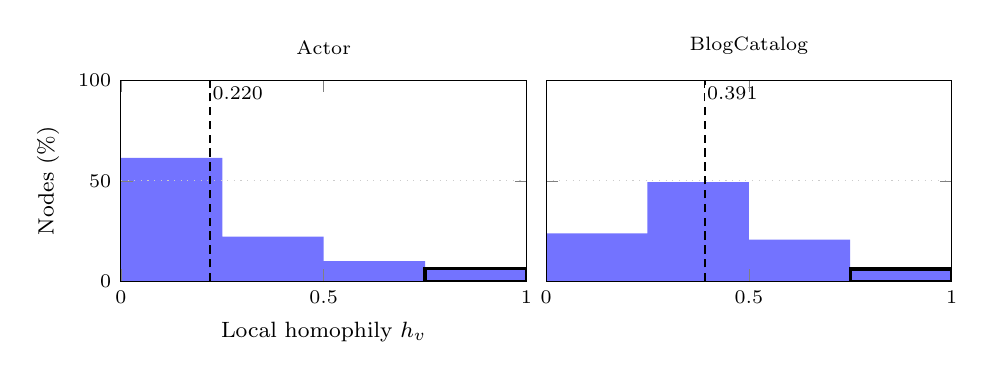
\begin{tikzpicture}
\begin{groupplot}[
    group style={
        group size=2 by 1,
        horizontal sep=0.25cm,
        ylabels at=edge left,
        yticklabels at=edge left
    },
    scale only axis,
    width=5.15cm,
    height=2.55cm,
    xmin=0, xmax=1,
    ymin=0, ymax=100,
    xtick={0,0.5,1},
    ytick={0,50,100},
    tick label style={font=\scriptsize},
    title style={font=\scriptsize},
    label style={font=\footnotesize},
    ymajorgrids=true,
    grid style={dotted,gray!40},
    axis on top,
]

\nextgroupplot[
    title={Actor},
    ylabel={Nodes (\%)},
    xlabel={Local homophily \(h_v\)},
]
\addplot+[ybar interval, fill=blue!55, draw=none, mark=none]
coordinates {
    (0,61.4)
    (0.25,22.2)
    (0.5,10.1)
    (0.75,6.3)
    (1,0)
};
\addplot+[ybar interval, fill=blue!55, draw=black, line width=1.2pt, mark=none]
coordinates {(0.75,6.3) (1,0)};
\draw[densely dashed,black,line width=0.7pt]
    (axis cs:0.220,0) -- (axis cs:0.220,100);
\node[font=\scriptsize,anchor=north west,fill=white,inner sep=0.7pt]
    at (axis cs:0.220,98) {0.220};

\nextgroupplot[title={BlogCatalog}]
\addplot+[ybar interval, fill=blue!55, draw=none, mark=none]
coordinates {
    (0,23.8)
    (0.25,49.4)
    (0.5,20.8)
    (0.75,6.1)
    (1,0)
};
\addplot+[ybar interval, fill=blue!55, draw=black, line width=1.2pt, mark=none]
coordinates {(0.75,6.1) (1,0)};
\draw[densely dashed,black,line width=0.7pt]
    (axis cs:0.391,0) -- (axis cs:0.391,100);
\node[font=\scriptsize,anchor=north west,fill=white,inner sep=0.7pt]
    at (axis cs:0.391,98) {0.391};

\end{groupplot}
\end{tikzpicture}
\caption{Distribution of nodes across local-homophily bins. Bar
widths show the bin intervals and heights show within-dataset percentages.
Dashed lines give mean \(h_v\); thick outlines mark the selected tails.}
\label{fig:additional-local-homophily-bins-tikz}
\end{figure}
